% \documentclass[uplatex,dvipdfmx,11pt,a4paper,twoside]{jsreport}
% \usepackage{mypackage}

% \begin{document}
%%%%%%%%%%%%%%%%%%%%%%%%%%%%%%%%%%%%%
\chapter{序論}
\section{セクション}
\subsection{サブセクション}
参考文献は、論文\cite{sample-2}、書籍\cite{totto2023}、その他\cite{sample}としてref.bibに記述すると良い。
論文であれば、多くの場合bibtex出力が可能であり、bibtexがない場合でもhoge.risとして出力が可能である。
hoge.risの場合は、hoge.risから.bibに変換するサービスがおんらいんであるのでそれを利用すると良い。

段片はこのようにする。
このようにしても変わらない。

図は、図\ref{texwiki}と参照できるし、mypackage.styをusepackageしていれば、「図」を直打ちせずに\fref{texwiki}とすればよい。
ソースファイルとpdfを見比べると何言っているか分かる。

\clearpage

\begin{figure}[htbp]
  \centering
  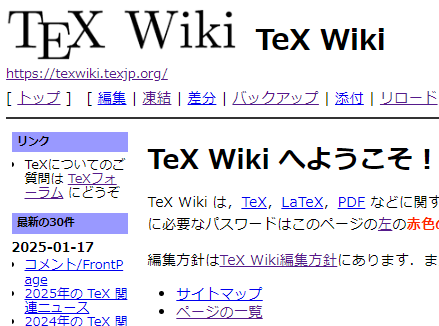
\includegraphics[width=.6\linewidth]{fig/sample.png}
  \caption{\TeX 初心者はよくお世話になるサイトになると思われる\href{https://texwiki.texjp.org}{\bf site here!}}
  \label{texwiki}
\end{figure}

% \end{document}